%\documentclass[10pt]{letter}
%\usepackage[utf8]{inputenc}

%%%%%%%%%%%%%%%%%%%%%%%%%%%%%%%%%%%%%%%%%%%%%%%%%
% compile with LuaLatex
%%%%%%%%%%%%%%%%%%%%%%%%%%%%%%%%%%%%%%%%%%%%%%%%%%%%%%%
\documentclass[11pt]{report}
\usepackage{epsfig}
\usepackage{amssymb,amsmath,amsfonts}
\usepackage[activeacute,american]{babel}
%\usepackage[utf8]{inputenc}
\usepackage{subfiles}
\usepackage{cite}
\usepackage{csquotes}
\usepackage{esvect}
\usepackage[acronym,nonumberlist]{glossaries}
\renewcommand{\acronymname}{Nomenclature}
\usepackage{multicol}
\usepackage{caption} 
\usepackage{float}
\usepackage[
    math-style=ISO,      % Upper Case Greek is in italics
    bold-style=ISO,      % Bold math is in italics
    partial=upright,     % nabla and partial upright
    nabla=upright,
  ]{unicode-math}
\topmargin 1.2cm 
\textwidth 16.1cm
\textheight 22.5cm
\oddsidemargin 0.7cm
\setcounter{tocdepth}{5}
\addtolength{\voffset}{-2.4cm}
\addtolength{\hoffset}{-0.5cm}

\usepackage{setspace}
%\doublespacing
\onehalfspacing
\usepackage{caption}
 \captionsetup[figure]{labelfont={bf},name={Figura},labelsep=period}


%%%%%%%%%%%%%%%%%%%%%%%%%%%%%%% 
% citas
% \footnotetext{Mott, Robert L. Mecanica de Fluidos 6/e. Pearson educación, 2006.}
% \footnotetext{Pritchard, Philip J. Fox and McDonald’s Introduction to Fluid Mechanics (8th ed.). John Wiley $\&$ Sons. (2011).}
% \footnotetext{Munson, Bruce R., et al. "Fundamentals of Fluid Mechanics, John Wiley $\&$ Sons." Inc., USA (2006).}
%%%%%%%%%%%%%%%%%%%%%%%%%%%%%%% 

%%%%%%%%%%%%%%%%%%%%%%%%%%%%%%%%%
\begin{document}
\centering{ \textbf{\Large{Mec\'anica de fluidos}}}

\vspace{1cm}

\flushleft{ \large \underline{\textbf{Pr\'actica 4: Ecuaci\'on de Bernoulli}}}

%%%%%%%%%%%%%%%%%%%%%%%%%
\vspace{1cm}

\underline {Problema 1 (P. 6.61M Mott\footnote{footnotes working fine}):}

\vspace{0.2cm}

En la tuber\'ia presentada en la figura~\ref{fig:fig1} fluye agua a $10$\,$^\circ$C, a raz\'on de $0.37$\,m$^3$/s. Si la presi\'on en el punto A es de $66.2$\,kPa, calcule la presi\'on en el punto B.

\vspace{0.2cm}

\underline {Problema 2 (P. 6.62M Mott):}

\vspace{0.2cm}

Calcule el flujo volum\'etrico de agua a $5$\,$^\circ$C que pasa por el sistema ilustrado en la figura~\ref{fig:fig2}


\begin{multicols}{2}
\begin{figure}[H]
\centering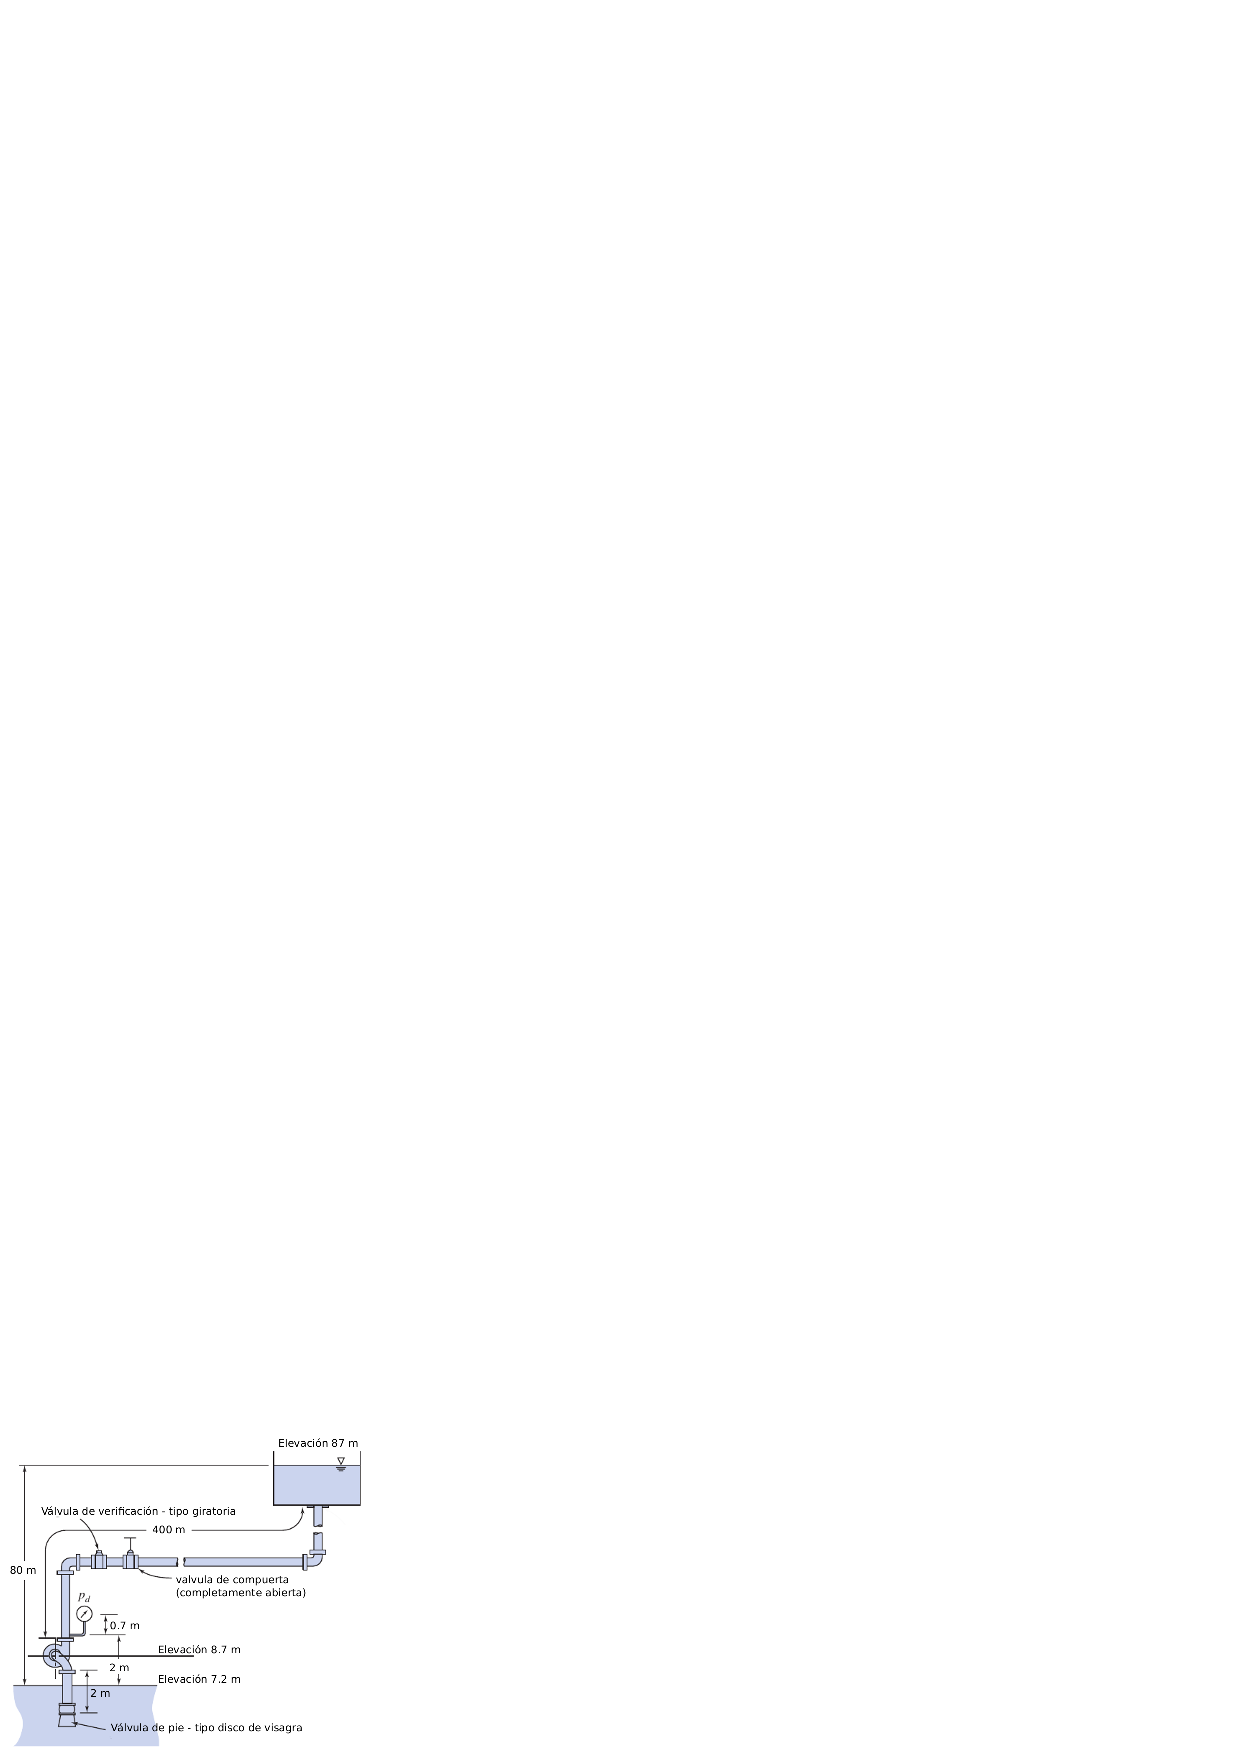
\includegraphics[width=0.4\textwidth]{p1.png}
\caption{\label{fig:fig1} }
\end{figure}
\columnbreak
\vspace*{\fill}
\begin{figure}[H]
\centering\includegraphics[width=0.4\textwidth]{p2.png}
\caption{\label{fig:fig2}}
\end{figure}
\end{multicols}

\footnotetext{Mott, Robert L. Mecanica de Fluidos 6/e. Pearson educación, 2006.}

%%%%%%%%%%%%%%%%%%%%%%%%%
\newpage
%%%%%%%%%%%%%%%%%%%%%%%%%
\vspace{1cm}

\underline {Problema 3 (P. 6.65M Mott):}

\vspace{0.2cm}

Para el sistema mostrado en la figura~\ref{fig:fig3}, calcule:\newline

a) El flujo volum\'etrico de agua que sale de la tobera\newline
b) La presi\'on en el punto A

\begin{figure}[H]
\centering\includegraphics[width=0.45\textwidth]{p3.png}
\caption{\label{fig:fig3} }
\end{figure}

%%%%%%%%%%%%%%%%%%%%%%%%%
\underline {Problema 4 (P. 6.72M Mott):}

\vspace{0.2cm}

Para el sif\'on de la figura~\ref{fig:fig4}, calcule:\newline

a) El flujo volum\'etrico de aceite que sale del tanque\newline
b) Las presiones en los puntos A y D

\begin{figure}[H]
\centering\includegraphics[width=0.45\textwidth]{p4.png}
\caption{\label{fig:fig4}}
\end{figure}


%%%%%%%%%%%%%%%%%%%%%%%%%

\underline {Problema 5 (P. 6.75M-6.76M Mott):}

\vspace{0.2cm}

En la figura~\ref{fig:fig5}, se muestra un man\'ometro que se emplea para medir la diferencia de presi\'on entre dos puntos en un sistema de tuber\'ia. \newline

a) Calcule el flujo volum\'etrico del agua en el sistema, si la diferencia de alturas $h$ en el man\'ometro es de $250$\,mm.\newline
b) Calcule la diferencia de alturas $h$ en el manometro si la velocidad de flujo de agua en la secci\'on de $25$\,mm de di\'ametro es de $10$\,m/s.

 
\begin{figure}[H]
\centering\includegraphics[width=0.5\textwidth]{p5.png}
\caption{\label{fig:fig5}}
\end{figure}


%%%%%%%%%%%%%%%%%%%%%%%%%

\underline {Problema 6 (P. 6.78M Mott):}

\vspace{0.2cm}

El medidor venturi de la figura~\ref{fig:fig6} conduce aceite ($SG=0.9$) la gravedad espec\'ifica del fluido en el man\'ometro es de $1.4$. Calcule el flujo volum\'etrico del aceite.

\begin{figure}[H]
\centering\includegraphics[width=0.3\textwidth]{p6.png}
\caption{\label{fig:fig6}}
\end{figure}

%%%%%%%%%%%%%%%%%%%%%%%%%
\newpage 
\underline {Problema 7 (P. 6.79M - 6.80M Mott):}

\vspace{0.2cm}
A trav\'es del medidor venturi de la figura~\ref{fig:fig7} fluye hacia abajo aceite con gravedad espec\'ifica de $0.9$. \newline

a) Si la deflexi\'on del man\'ometro $h$ es de $28$\,in, calcule el flujo volum\'etrico de aceite. \newline
b) Si la velocidad del flujo en la secci\'on de $2$\,in de diametro es de $10.0$\,ft/s, calcule la deflexi\'on $h$ del man\'ometro.
\begin{figure}[H]
\centering\includegraphics[width=0.7\textwidth]{p7.png}
\caption{\label{fig:fig7}}
\end{figure}
%%%%%%%%%%%%%%%%%%%%%%%%%
\newpage 
\underline {Problema 8 (P. 6.91M Mott):}
En la figura~\ref{fig:fig8} se presenta un estanque con un agujero por el cual fluye un chorro de agua. Calcule la altura m\'axima que puede alcanzar el chorro.

\begin{figure}[H]
\centering\includegraphics[width=0.45\textwidth]{p8.png}
\caption{\label{fig:fig8}}
\end{figure}
%%%%%%%%%%%%%%%%%%%%%%%%%
\underline {Problema 9 (P. 6.92E Mott):}
En la figura~\ref{fig:fig9} se presenta un estanque con un agujero por el cual fluye un chorro de agua. Calcule la altura m\'axima que puede alcanzar el chorro.

\begin{figure}[H]
\centering\includegraphics[width=0.45\textwidth]{p9.png}
\caption{\label{fig:fig9}}
\end{figure}


%%%%%%%%%%%%%%%%%%%%%%%%%
%%%%%%%%%%%%%%%%%%%%%%%%%
%%%%%%%%%%%%%%%%%%%%%%%%%
\end{document}
